\section{MVE -- \emph{Multi-View Reconstruction Environment}}\label{sec:mve}
%======================================================================================
%
\subsection*{Introdução}
Um dos algoritmos utilizados para a técnica de reconstrução densa é o MVE -- \emph{Multi-View Reconstruction Environment}~\cite{mve}. Este algoritmo utiliza fotos e produz uma malha triangular superficial como resultado. Diferentemente das reconstruções baseadas nas geometrias das imagens, o MVE é focado na reconstrução multi-escala, um quesito importante na reconstrução de esculturas e acervo cultural. Portanto, com esta técnica é possível reconstruir grandes volumes de dados, contendo regiões detalhadas em alta resolução, em comparação com o resto da cena. O sistema ainda possui uma interface gráfica para o uma reconstrução baseada no SfM, amigável ao usuário (conhecida como UMVE), onde permite a visualização e inspeção das imagens, mapas de profundidade e renderizar cenas e malhas 3D.

Sua base de operação é basicamente \ref{fig:mvepipeline}:

\begin{enumerate}
\item{Estrutura da formação -- \emph{Structure-from-Motion} (SfM)}

\begin{itemize}
\item{
Reconstrói os parâmetros da câmera (posição e orientação) e seus dados de calibração (distância focal e distorção radial),
encontrando correspondências esparsas, mas estáveis entre as imagens.
}
\end{itemize}

\item{Múltiplas visões estéreo -- \emph{Multi-View Stereo} (MVS)}
\begin{itemize}
\item{
Utiliza a posição estimada das câmeras, encontrando as correspondências visuais nas imagens. Estas correspondências são trianguladas, produzindo a informação 3D, e,
consequentemente a reconstrução 3D densa.
} 
\end{itemize}
\item{Reconstrução de superfícies -- \emph{Surface Reconstruction}}
\begin{itemize}
\item{
Tem como entrada uma densa nuvem de pontos, ou mapas de profundidade individuais. Produz uma malha superficial globalmente consistente.
}
\end{itemize}
\end{enumerate}

\begin{figure}[!h]
	\centering
	%   \includegraphics[width=1.0\linewidth]{figs/3d-curve-sketch/system-diagram.eps}
	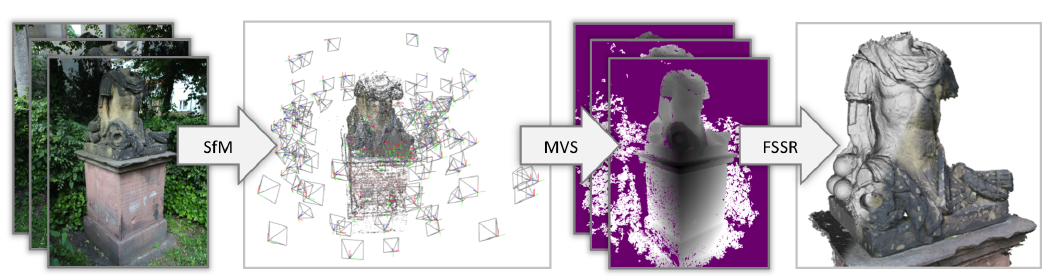
\includegraphics[width=0.8\linewidth]{figs/mvepipe.png}
	\caption{%
	Funcionamento do MVE. Começando com múltiplas imagens, técnicas SfM são empregadas para recontruir os parâmetros das câmeras e os conjuntos de pontos esparsos. Mapas de profundidade são computados para cada imagem usando o MVS. Finalmente, uma malha colorida é extraída da união de todos os mapas de profundidade usando um algoritmo de aproximações de reconstruções de superfícies (FSSR -- \emph{Floating Scale Surface Reconstruction}).
	\protect\cite{mve}
	}\label{fig:mvepipeline}
\end{figure}

Como não existem muitas opções para algoritmos de SfM, o MVE permite a utilização de \emph{softwares} externos como o \emph{Bundler}~\cite{snavely2010bundler} ou o prório \emph{VisualSfM}.

Uma vez com o passo do SfM feito, partimos para o MVS. Com os parâmetros de câmera conhecidos, a reconstrução densa geométrica é feita. Existem diversos algoritmos para a reconstrução densa, o MVE no caso, utiliza um algoritmo próprio, feito por um de seus criadores, Michael Goesele~\cite{goesele2007multi}, que reconstrói um mapa de profundidade para cada foto. 

Embora abordagens baseadas em mapeamentos de profundidade produzam uma grande quantidade de redundâncias, (isso se dá por causa das inúmeras fotos que são sobrepostas e possuem partes similares da mesma cena), este algoritmo é altamente escalável para grandes cenas, pois apenas um pequeno conjunto de fotos vizinhas é necessário para a reconstrução. Outra vantagem da utilização dos mapas de profundidade como representação intermediária é que a geometria é parametrizada em seu domínio natural, e os dados por foto (como a cor, por exemplo) estão diretamente acessíveis nas imagens.

Essa redundância excessiva nos mapas de profundidade pode ser pesado. Não com relação ao armazenamento, mas na questão do processamento computacional exigido nos mapas. Porém, esta abordagem foi capaz de produzir uma geometria detalhada e superar o ruído nos mapas de profundidade individuais.

\subsection*{Guia de reconstrução com o MVE}
Existem algumas recomendações para se ter uma boa reconstrução com o MVE~\cite{pipelinemve,mve}.
Um bom conjunto de dados é gerado se algumas regras simples forem seguidas:

\begin{itemize}

\item{Para que o algoritmo do MVS consiga fazer uma triangulação com qualquer posição 3D, o conjunto de dados terá que ter, no mínimo, cinco fotos.}

\item{As fotos devem ser tiradas com uma boa quantidade de sobreposição. A menos que o conjunto de dados se torne muito grande, uma grande quantidade de fotos não prejudicará a qualidade. 
Mas terá uma compensação do sistema, no que diz respeito à qualidade e desempenho.}

\item{Para a triangulação funcionar, é necessário que tenha o efeito de paralaxe \ref{fig:parallax} (Aparente mudança na posição do objeto). Ou seja, é interessante que o conjunto de imagens seja duplicado.}

\item{A câmera deverá ser reposicionada, de preferência.}

\end{itemize}

\begin{figure} [!h]
	\centering
	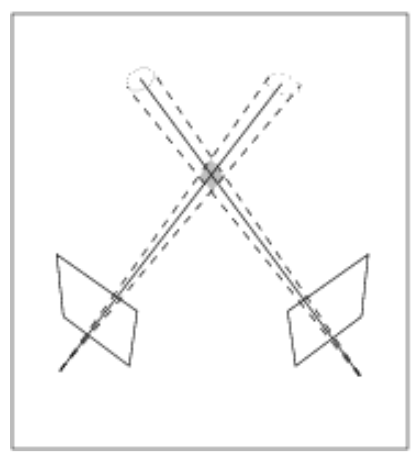
\includegraphics[width=0.2\linewidth]{figs/parallaxA.png}(a)
	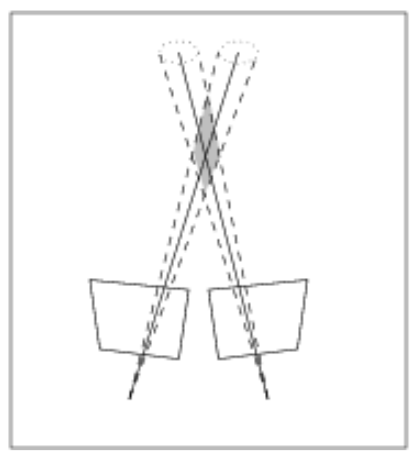
\includegraphics[width=0.2\linewidth]{figs/parallaxB.png}(b)
	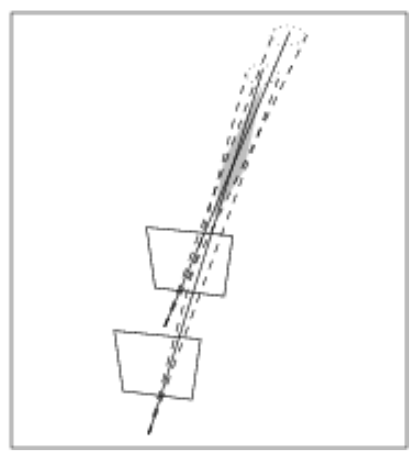
\includegraphics[width=0.2\linewidth]{figs/parallaxC.png}(c)
	\caption{%
	Caso o espaçamento entre as câmeras seja grande, a informação extraída das imagens em comum será menor (a). Se a angulação do efeito de paralaxe seja baixa, terá a mesma informação sobre um ponto em questão (c). Ou seja utilizando ou (a), ou (c). Pode ser que a reconstrução fique incerta. Para que o efeito paralaxe tenha maior proveito das imagens das câmeras, é necessário que as câmeras estejam dispostas como (b), conseguindo extrair uma boa quantidade e qualidade de informações do ponto.
	\protect\cite{3DCompVision2Didier}
	}
	\label{fig:parallax}
\end{figure}

% Creating a scene: A view is a container that contains per-
% viewport data (such as images, depth maps and other data).
% A scene is a collection of views, which make up the dataset.
% A new scene is created using either the graphical interface of
% our software, UMVE, or the command line tool makescene.
% Technically, the scene appears as a directory in the file sys-
% tem (with the name of the dataset). It contains another direc-
% tory views/ with all views stored as files with the extension
% .mve. Creating a new scene will solely create the views/
% directory for now. Importing photos will create a .mve file
% for every photo. This process will also import meta informa-
% tion from the images (EXIF tags), which is required to get
% a focal length estimate for every photo. If EXIF tags are not
\subsubsection*{Criando uma cena}

Uma visualização contém dados por exibição (como imagens, mapas de profundidade ou outros dados). Uma cena é uma coleção de visualizações, que constitui um conjunto de dados. Uma nova cena pode ser criada utilizando a interface gráfica UMVE, ou por linha de comando (\emph{makescene}). 

Tecnicamente, a cena é criada como um diretório no sistema de arquivos (com o nome do conjunto de dados). Este, por sua vez, contém outro diretório (\emph{views}), com todas as visualizações guardadas com uma extensão de arquivos em .MVE.

Criar uma nova cena, criará apenas o diretório (\emph{views}) vazio. A importação de fotos criará arquivos .MVE para cada foto. Esse processo importará meta-dados provenienteas das imagens (\emph{tags} EXIF), que é necessário para estimar a distância focal para cada foto. Caso estes meta-dados não estejam disponíveis, uma distância focal padrão é assumida pelo sistema, porém se essa distância adotada for uma péssima suposição, com relação ao conjunto de dados utilizado, pode vir a acontecer erros no SfM.

\begin{figure}[!h]
	\centering
	%   \includegraphics[width=1.0\linewidth]{figs/3d-curve-sketch/system-diagram.eps}
	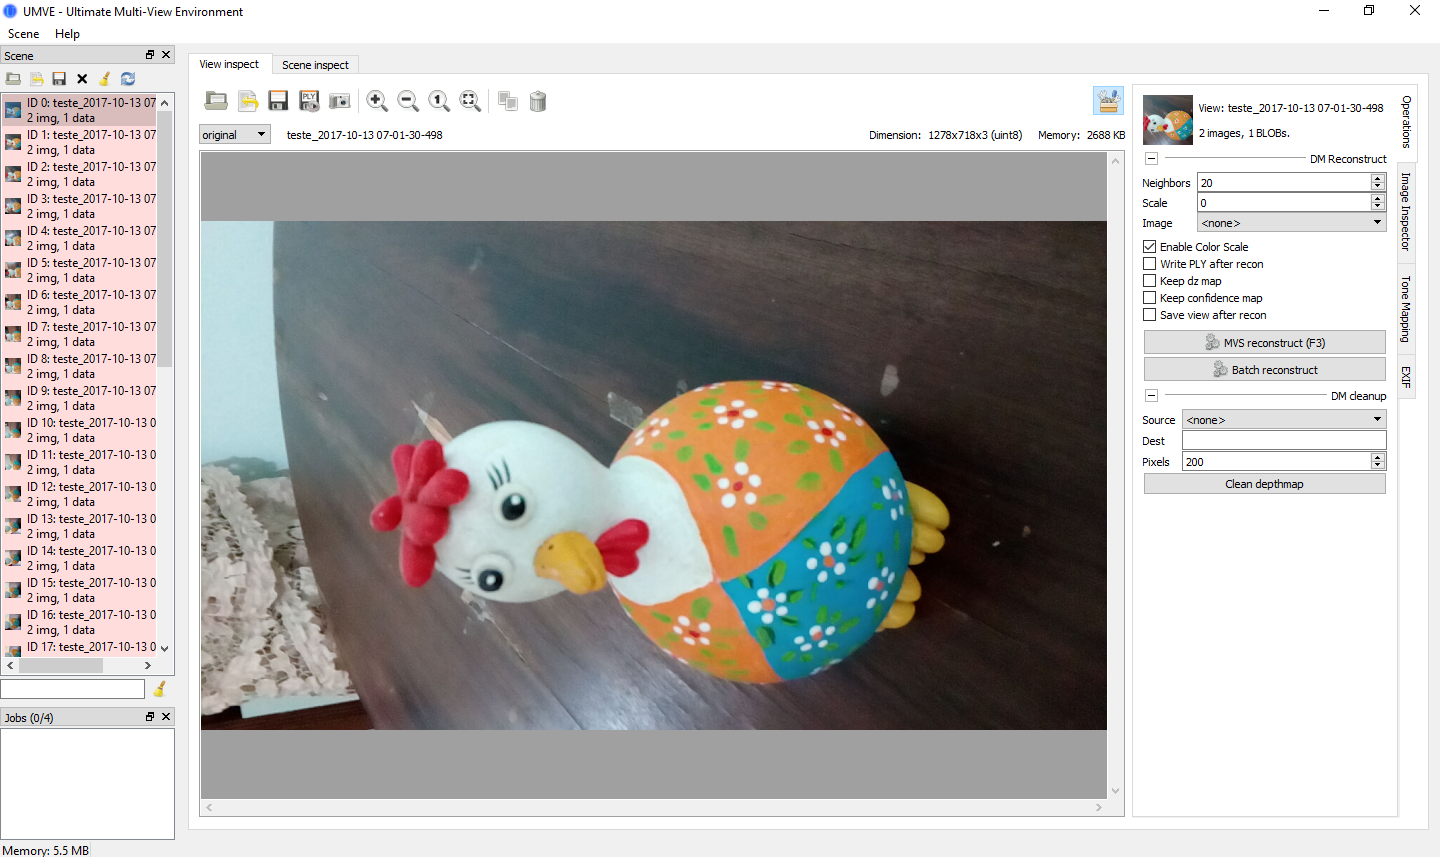
\includegraphics[width=0.7\linewidth]{figs/umve1.png}
	\caption{%
	Interface gráfica (UMVE)%\cite{Cui:Theobalt:etal:PAMI2013,Pajdla:etal:ICCV2011}.
	}\label{fig:mvesfm}
\end{figure}
% SfM reconstruction: The SfM reconstruction can be con-
% figured and started using UMVE, or the command line tool
% sfmrecon. The UI guides through feature detection, pairwise
% matching and incremental SfM. What follows is the SfM re-
% construction starting from an initial pair, and incrementally
% adding views to the reconstruction. Finally, the original im-
% ages are undistorted and stored in the views for the next step.
% Figure 8 shows a rendering of the SfM reconstruction with
% the sparse point cloud and the camera frusta. Note how dense
% the frusta are spaced around the object to achieve a good re-
% construction.
\subsection*{Reconstrução SfM}

Pode ser configurada e iniciada usando a interface gráfica UMVE ou por linha de comando (\emph{sfmrecon}). A interface guia através da detecção de \emph{features}, combinação emparelhada (\emph{pairwise matching}) e uso incremental do SfM. Que, por sua vez, a reconstrução SfM começa a partir de um par inicial, e adiciona, de forma incremental, mais vistas à reconstrução \ref{fig:mvesfm}.

\begin{figure}[!h]
	\centering
	%   \includegraphics[width=1.0\linewidth]{figs/3d-curve-sketch/system-diagram.eps}
	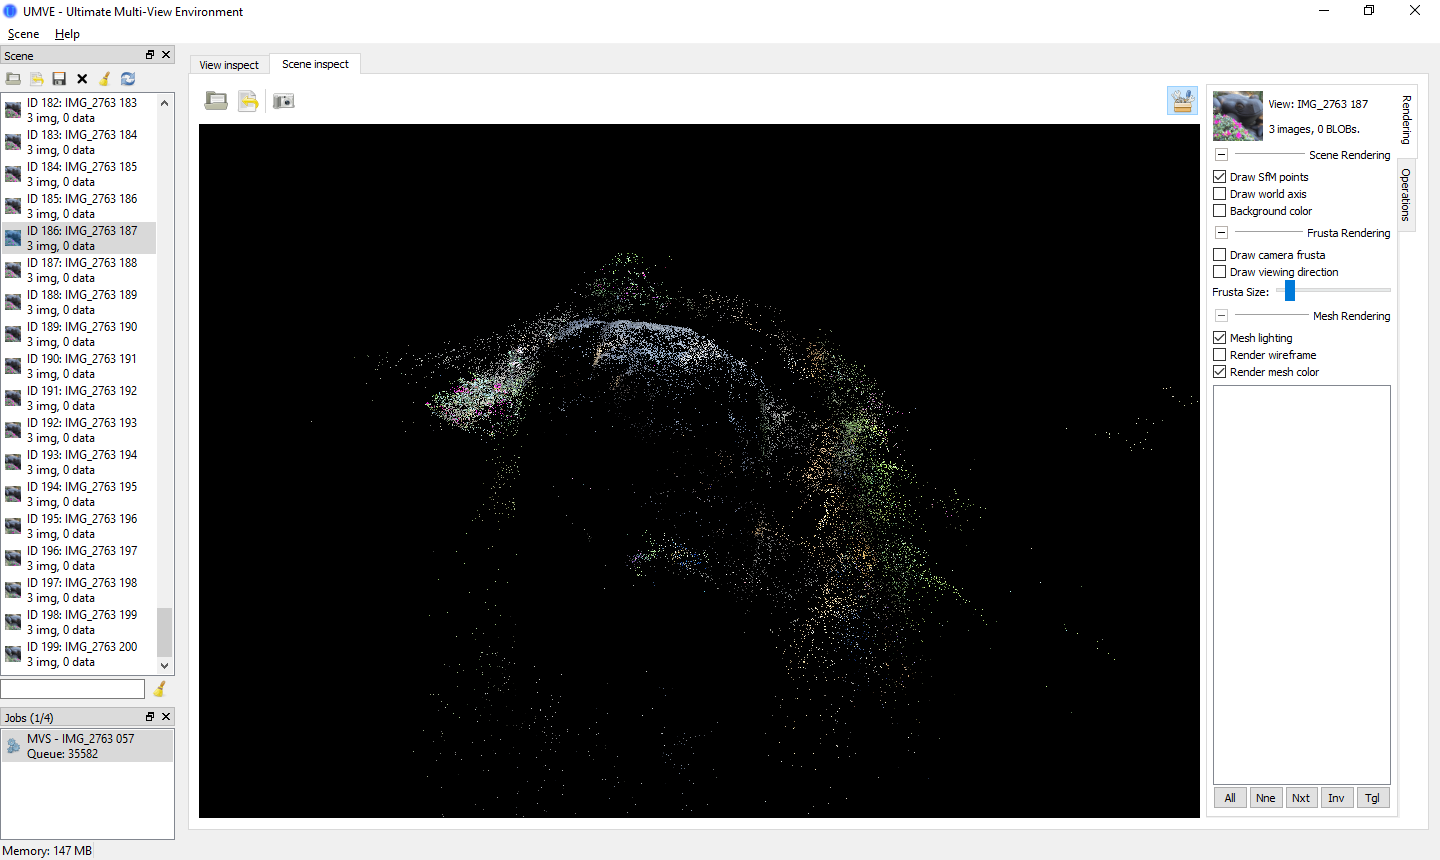
\includegraphics[width=0.7\linewidth]{figs/umve5sfm.png}
	\caption{%
	Reconstrução baseada em nuvem de pontos gerada a partir da reconstrução SfM.%\cite{Cui:Theobalt:etal:PAMI2013,Pajdla:etal:ICCV2011}.
	}\label{fig:mvesfm}
\end{figure}


%
%MVS reconstruction: Given images with camera parameters,
%dense geometry is reconstructed using MVS. This can
%be done with either UMVE or the command line tool dmrecon.
%The most important parameter is the resolution level at
%which depth maps are reconstructed. A level of 0, or L0, reconstructs
%at the original image size, L1 corresponds to half
%the size (quarter the number of pixels), and so one. Looking
%at the resolution of recent digital cameras, a full-size L0
%reconstruction is rarely useful as finding dense correspondences
%gets more difficult, often leading to sparser depth
%maps at much higher computational cost. Using smaller images
%(we often use L2), the process is faster and depth maps
%become more complete. See Figure 9 for a depth map computed
%at L2.
\subsubsection*{Múltiplas visões estéreo -- \emph{Multi-View Stereo} (MVS)}

Usando as imagens junto com os parâmetros obtidos das câmeras, é possível reconstruir a geometria densa utilizando o MVS. Isso pode ser feito utilizando a interface gráfica (UMVE) ou por linha de comando (\emph{dmrecon}).

O parâmetro mais importante é o nível de resolução em que os mapas de profundidade são reconstruídos: Caso seja nível 0 (ou L0), a reconstrução é feita usando o tamanho original das imagens. Se for nível 1 (ou L1), a reconstrução corresponde a metade do tamanho (um quarto dos números de pixels), e assim por diante.

Com a resolução das câmeras atuais, uma reconstrução L0 é raramente usada, pois geram mapas de profundidade mais dispersos com um custo computacional elevado, o que acarreta em dificuldades para encontrar as correspondências densas das imagens. Geralmente utiliza-se o L2, pois o processo é mais rápido, gerando mapas de profundidades completos, já que utiliza imagens menores \ref{fig:mvedepth}.

\begin{figure}[!h]
	\centering
	%   \includegraphics[width=1.0\linewidth]{figs/3d-curve-sketch/system-diagram.eps}
	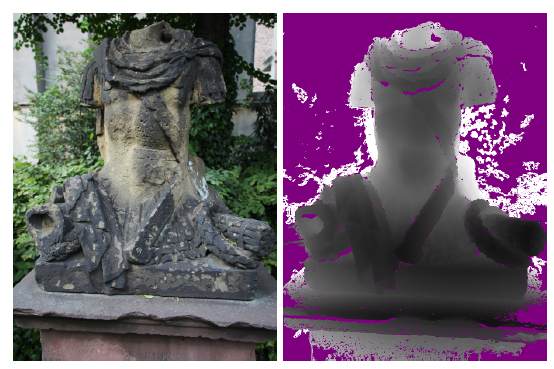
\includegraphics[width=0.4\linewidth]{figs/mvedepth.png}
	\caption{%
	Uma imagem de entrada (à esquerda) e sua correspondência em mapas de profundidade (à direita), onde a parte roxa significa que não foi encontrada nenhum mapa naquela região \protect\cite{mve}.
	}\label{fig:mvedepth}
\end{figure}

\subsubsection*{Reconstrução de superfícies -- \emph{Surface Reconstruction}}

Utiliza-se a linha de comando \emph{scene2pet}, que combina todos os mapas de profundidade em uma única e grande nuvem de pontos. Nesta fase, um valor de escala é atribuído a cada ponto, que indica o tamanho atual da região da superfície na qual o ponto foi mensurado. Esta informação adicional permite o uso de várias propriedades benéficas usando a abordagem de reconstrução de superfície usando FSSR~\cite{fuhrmann2014floating}.  
A seguir, as ferramentas FSSR calculam uma representação volumétrica de escala múltipla a partir dos pontos (na qual não precisa de nenhum ajuste de parâmetros explícitos) e uma malha final é extraída. Esta malha pode parecer desordenada devido à regiões não confiáveis e à componentes isolados, oriundos de medidas imprecisas. Logo, a malha é limpa, retirando pequenos componentes isolados e regiões não confiáveis da superfície. 

% Experiência com o MVE: A utilização do \emph{software} é bem intuitiva, seja por linha de comando ou pela interface gráfica (neste modo, fica mais fácil visualizar cada etapa da reconstrução). Amplamente configurável, podendo escolher a vizinhança, escala, manter o mapa de profundidade, ver os dados \emph{EXIF} de cada imagem, dentre outras configurações.

% Entretanto, para a aplicação proposta neste projeto, não é muito interessante, visto que ele utiliza a informação das câmeras (\emph{EXIF}) e das imagens e, como as imagens empregadas na reconstrução são, tecnicamente, vídeos cortados em determinados \emph{frames}, não é possível obter a informação das câmeras \ref{fig:mveexif}, logo o \emph{software} não tem tanta aplicabilidade neste caso, pois recai no problema dos parâmetros padrões adotados para as câmeras não serem bons o suficiente para estes conjuntos de dados, a menos que sejam tiradas fotos sequenciais de alguma escultura ou objeto que se deseja gerar a reconstrução densa, pois dessa forma, as informações necessárias das câmeras estarão armazenadas.

% \begin{figure}[!h]
% 	\centering
% 	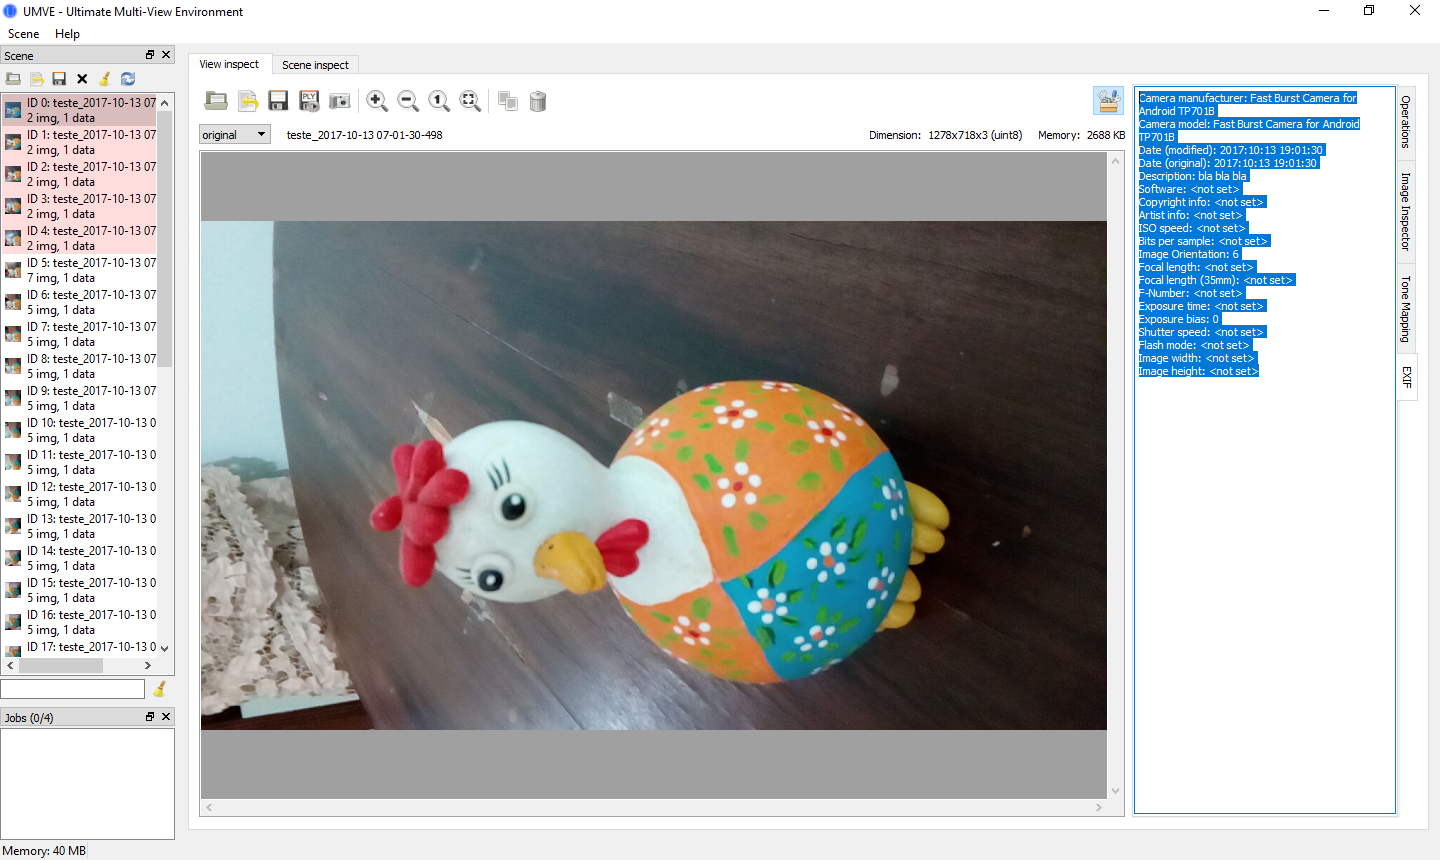
\includegraphics[width=0.5\linewidth]{figs/exifumve.png}(a)
% 	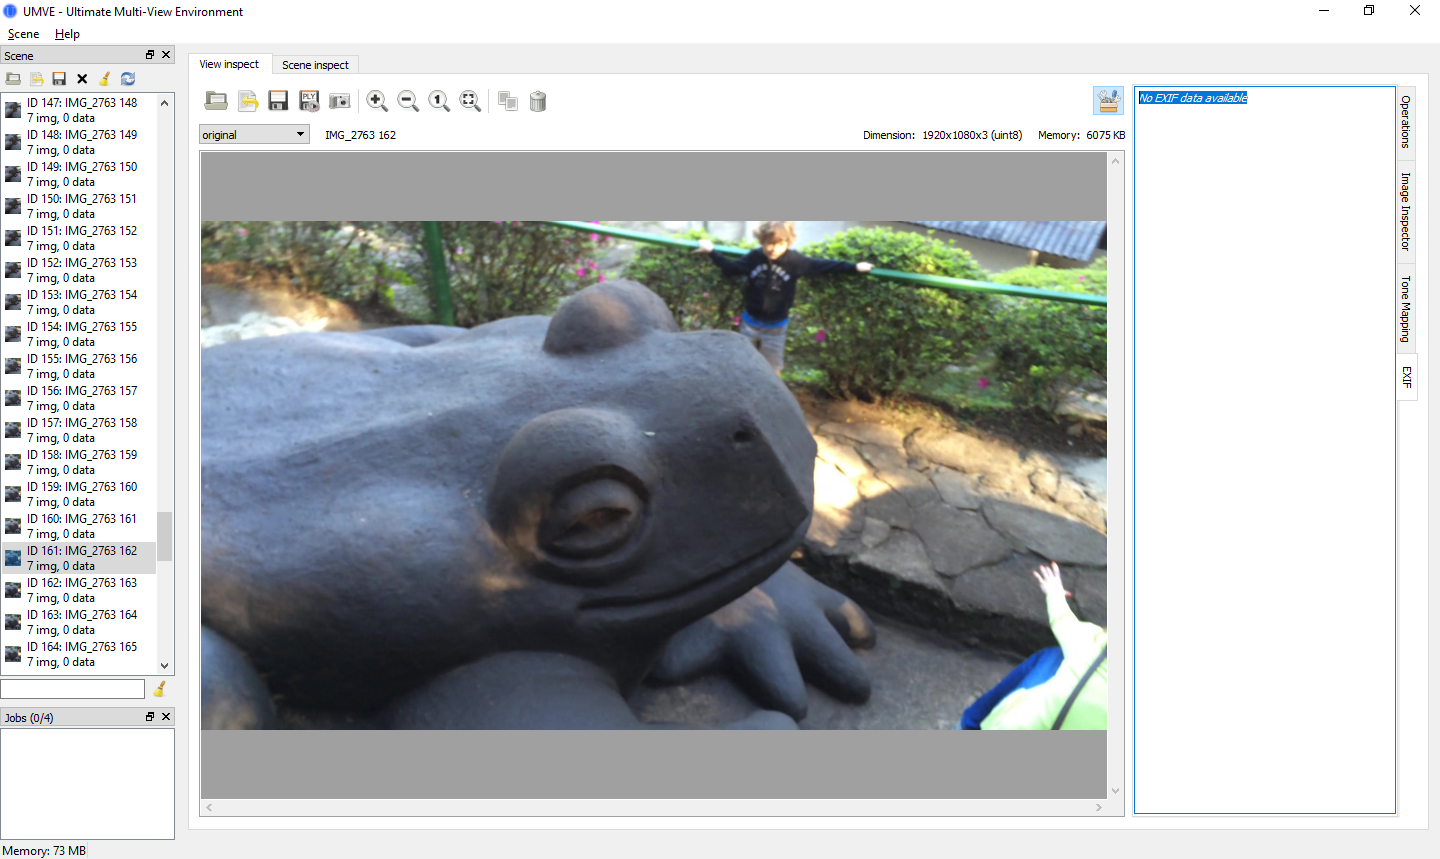
\includegraphics[width=0.5\linewidth]{figs/exifsemumve.png}(b)
% 	\caption{%
% 	A figura (a) é um exemplo onde a imagem possui dados na extensão \emph{EXIF} (destacado em azul). Ao passo que a figura (b) é um frame de um vídeo, que não possui os dados das câmeras (destacado em azul).
% 	%\cite{Cui:Theobalt:etal:PAMI2013,Pajdla:etal:ICCV2011}.
% 	}\label{fig:mveexif}
% \end{figure} 

% Com isso em mente, foi gerada uma reconstrução de um vídeo gravado de uma escultura no Jardim do Nêgo. O  vídeo foi cortado em \emph{frames} onde foram geradas 200 imagens base. 

% A partir disso, foi executado, todos os passos de uma reconstrução utilizando o MVE, de forma que, foram utilizadas as duas opções, tanto por linha de comando, quanto pela interface gráfica (UMVE).

% Pela interface gráfica, o processo todo de reconstrução foi rápido (cerca de 30 minutos) \ref{fig:UMVEdense}, ao passo que por linha de comando, levou cerca de 11 horas e 30 minutos. 

% O UMVE não sinaliza quando o processo em execução termina, então, a explicação para essa discrepância no tempo é devido à execução de outro comando, sobrepondo o que já estava sendo executado, sem deixar terminá-lo.

% \begin{figure}[!h]
% 	\centering
% 	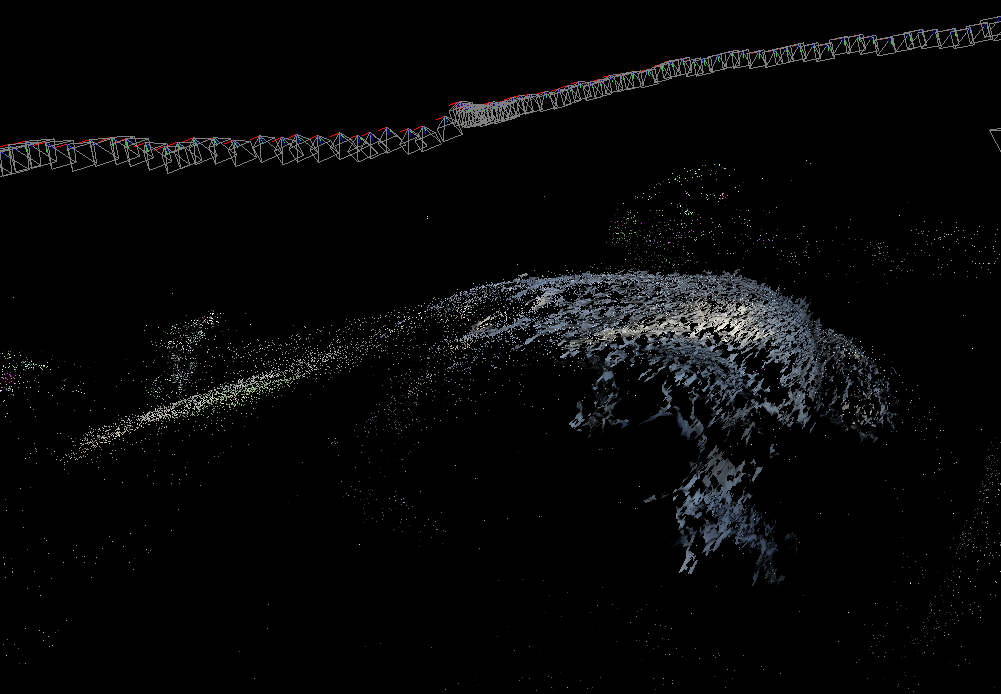
\includegraphics[width=0.5\linewidth]{figs/umvedense.png}
% 	\caption{%
% 	Final da reconstrução via UMVE, percebe-se que alguns pontos não foram considerados, tendo como resultado uma "nuvem de pontos" mais densa, basicamente.
% 	%\cite{Cui:Theobalt:etal:PAMI2013,Pajdla:etal:ICCV2011}.
% 	}\label{fig:UMVEdense}
% \end{figure} 

% Na reconstrução por linha de comando também é possível visualizar em qual etapa da execução o algoritmo está \ref{fig:passosMVE}, configurar alguns parâmetros e inclusive mostrar a porcentagem de progresso do comando. Foram executados os comandos declarados nesta seção.  O \emph{sfmrecon} demorou cerca de 1 minuto e meio \ref{fig:MVESfM}.

% \begin{figure}[!h]
% 	\centering
% 	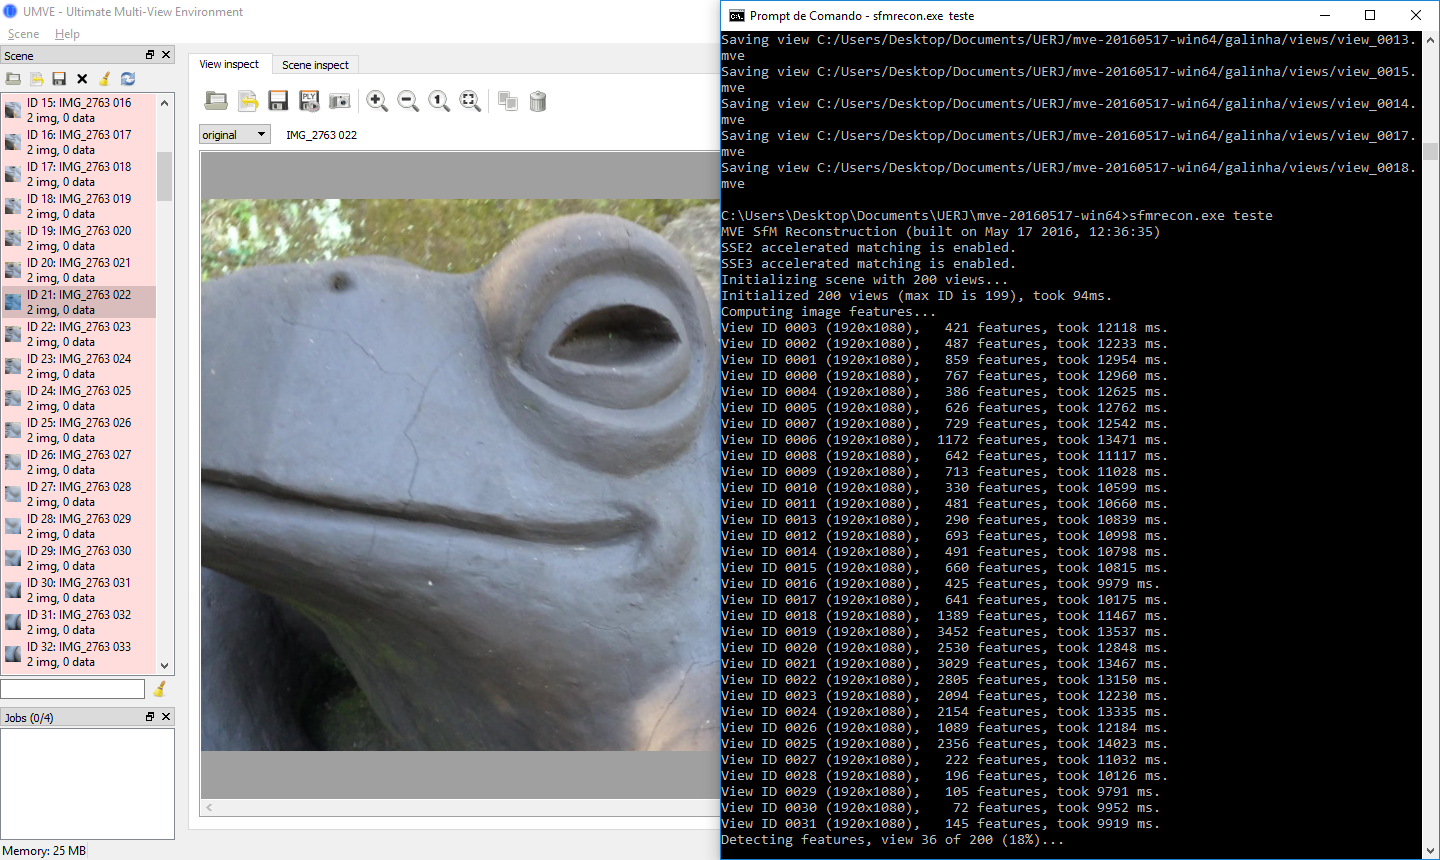
\includegraphics[width=0.5\linewidth]{figs/umve2sfm.png} (a)
% 	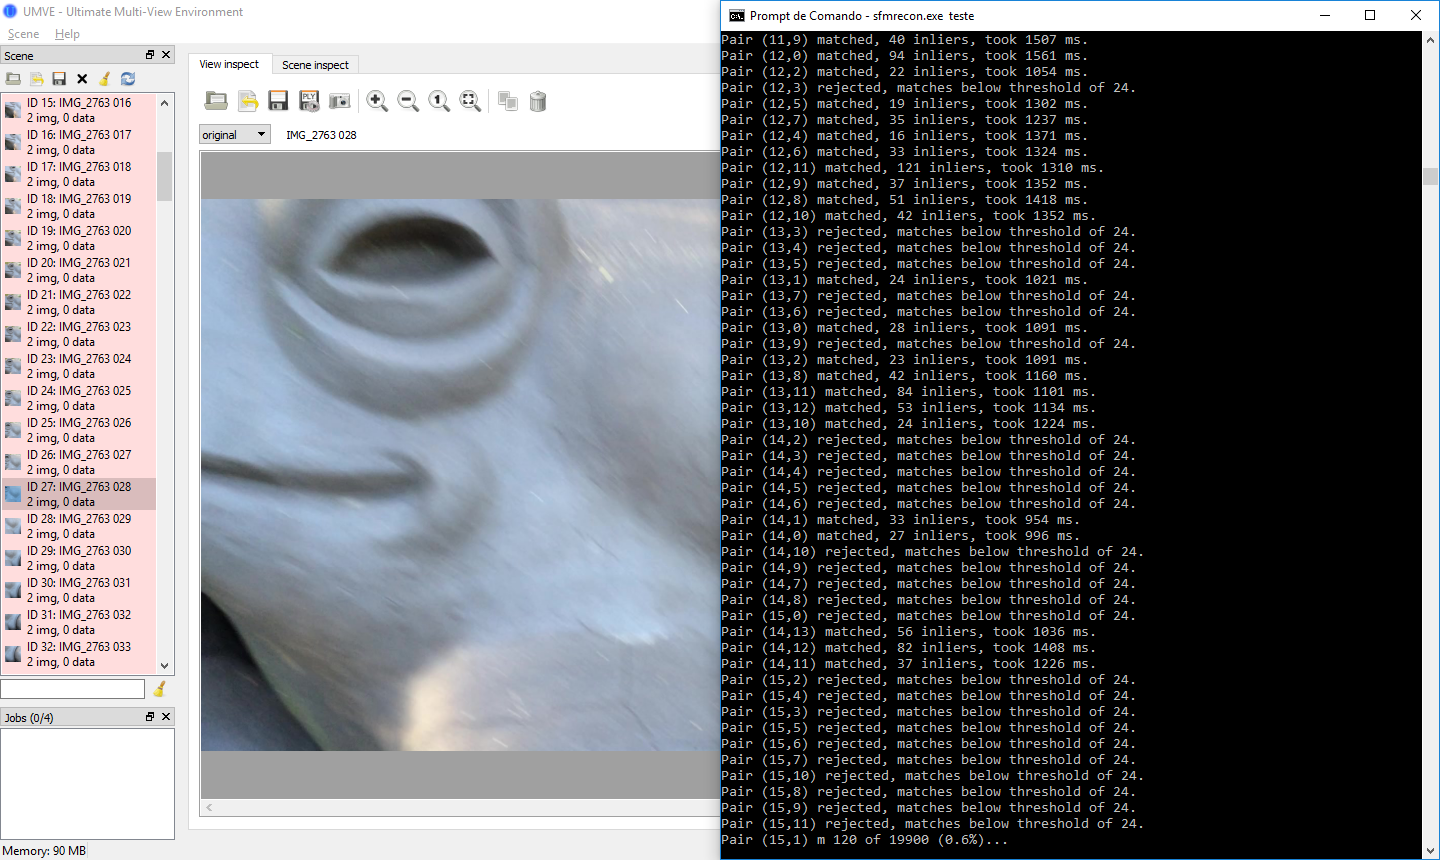
\includegraphics[width=0.5\linewidth]{figs/umve3sfmfeature.png} (b)
% 	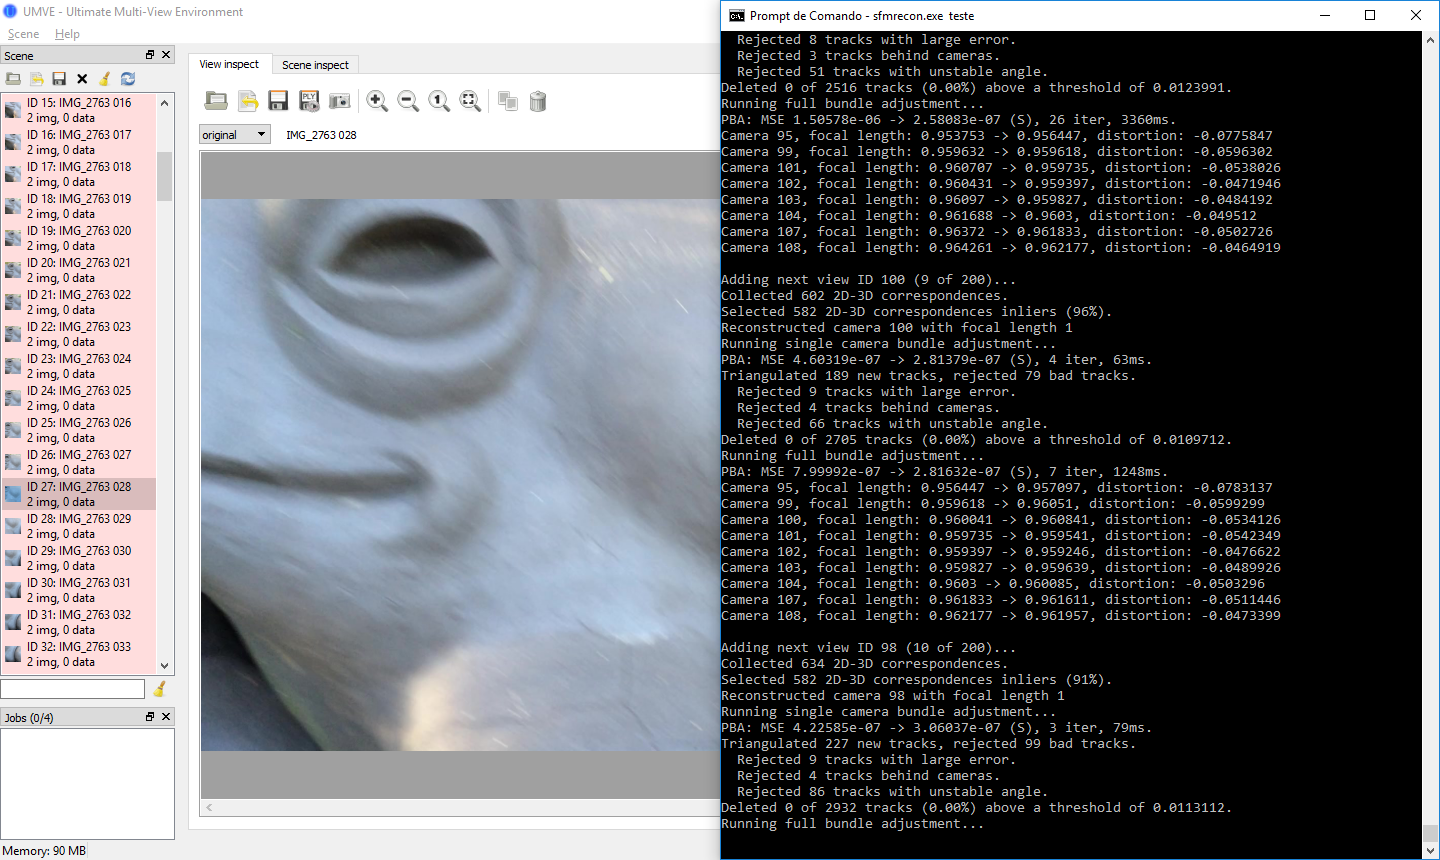
\includegraphics[width=0.5\linewidth]{figs/umve4ba.png} (c)
% 	\caption{%
% 	Processos dentro do comando \emph{sfmrecon}, onde (a) estão sendo detectadas as \emph{features} do conjunto de imagens. Em (b) está computado o \emph{pairwise matching} e em (c) está no processo de \emph{Bundle Adjustment}~\cite{bundleAdjustmentSlide}, usando condições-padrão para as câmeras.
% 	%\cite{Cui:Theobalt:etal:PAMI2013,Pajdla:etal:ICCV2011}.
% 	}\label{fig:passosMVE}
% \end{figure} 

% \begin{figure}[!h]
% 	\centering
% 	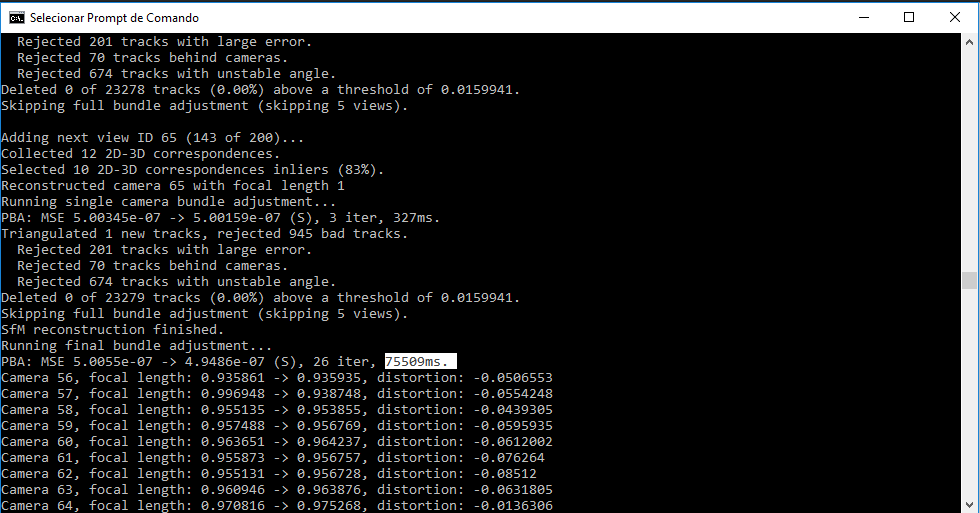
\includegraphics[width=0.8\linewidth]{figs/sfmmve.png}
% 	\caption{%
% 	Término do comando \emph{sfmrecon}, onde demorou cerca de 1 minuto e meio (75509 milisegundos).
% 	%\cite{Cui:Theobalt:etal:PAMI2013,Pajdla:etal:ICCV2011}.
% 	}\label{fig:MVESfM}
% \end{figure}

% O próximo comando, \emph{dmrecon} demorou cerca de 4 horas, usando como configuração um nível L2, com 20 vizinhos \ref{fig:MVEDenseRecon}. Usando um nível L0, o algoritmo rodou durante 6 horas aproximadamente e foi cancelado devido à demora na execução. 

% \begin{figure}[!h]
% 	\centering
% 	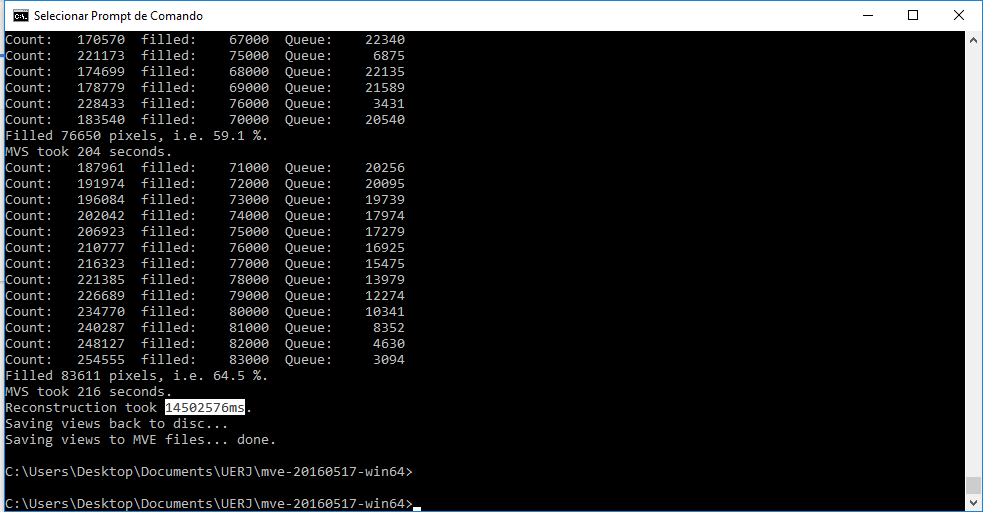
\includegraphics[width=0.8\linewidth]{figs/umvetempo.png}
% 	\caption{%
% 	Término do comando \emph{dmrecon}, onde demorou cerca de 4 horas (14502576 milisegundos).
% 	%\cite{Cui:Theobalt:etal:PAMI2013,Pajdla:etal:ICCV2011}.
% 	}\label{fig:MVEDenseRecon}
% \end{figure} 

% Usando o \emph{scene2pet}, é necessário em qual nível estamos reconstruindo e também uma saída válida. Por exemplo: "scene2pset.exe -Fnivel cena output". Onde o nível poderá ser um 0 (-F0), 1 (-F1) e assim por diante, a cena é o \emph{input} e o \emph{output} é um arquivo de extensão configurável, neste caso \emph{.ply} \ref{fig:MVEScene2Pet}. Este comando foi rápido, demorou cerca de 10 minutos, levando em conta todos os níveis.

% \begin{figure}[!h]
% 	\centering
% 	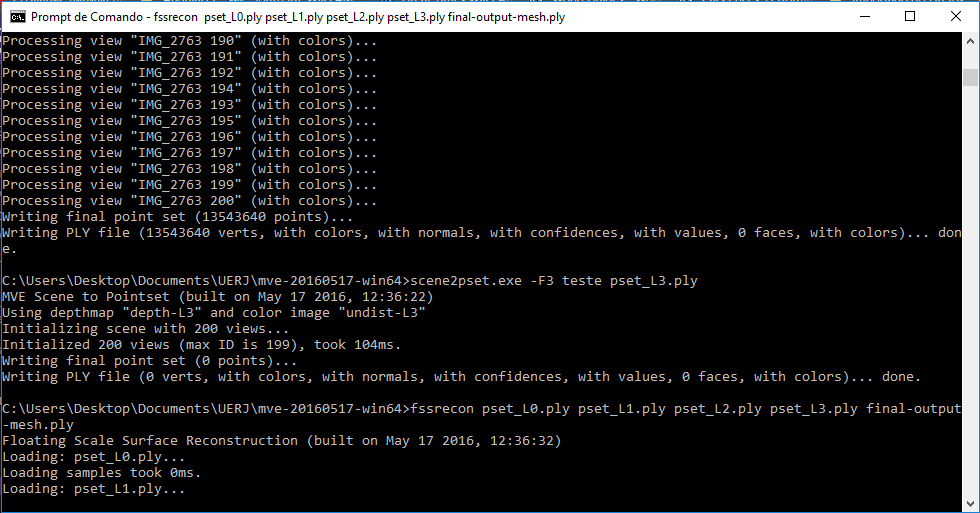
\includegraphics[width=0.8\linewidth]{figs/mvemesh.png}
% 	\caption{%
% 	Execução dos comandos \emph{scene2pet}, nos níveis -F0, -F1, -F2 e -F3.
% 	%\cite{Cui:Theobalt:etal:PAMI2013,Pajdla:etal:ICCV2011}.
% 	}\label{fig:MVEScene2Pet}
% \end{figure} 

% Para juntar todos os níveis do \emph{scene2pet}, foi usado o \emph{fssrecon}, que gera uma única reconstrução. Este processo demorou bastante, cerca de 7 horas \ref{fig:MVEFSSR}. Que teve como resultado a malha \ref{fig:MVEFSSRMesh}.

% \begin{figure}[!h]
% 	\centering
% 	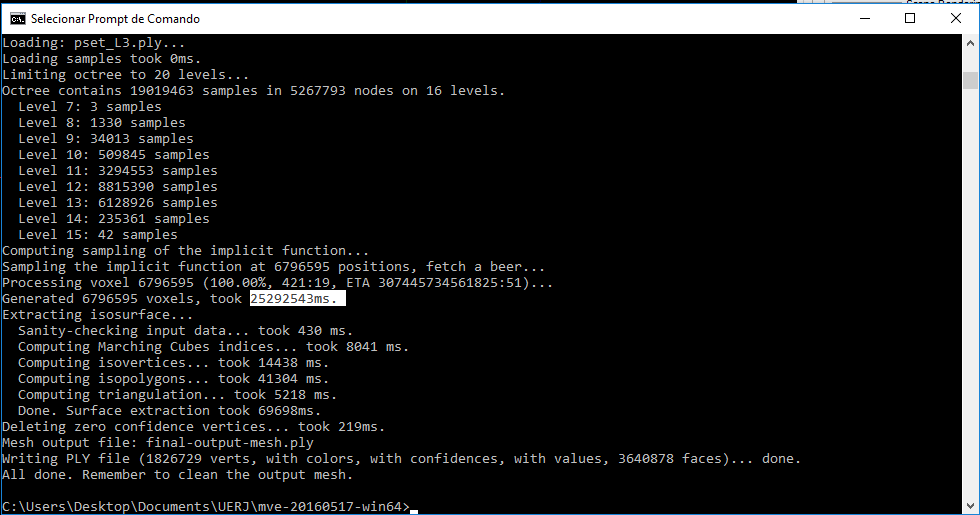
\includegraphics[width=0.8\linewidth]{figs/mvemeshtempo2.png}
% 	\caption{%
% 	Progressão do comando \emph{fssrecon}, onde possui o ETA -- \emph{Estimated Time of Arrival}.
% 	%\cite{Cui:Theobalt:etal:PAMI2013,Pajdla:etal:ICCV2011}.
% 	}\label{fig:MVEFSSR}
% \end{figure} 

% \begin{figure}[!h]
% 	\centering
% 	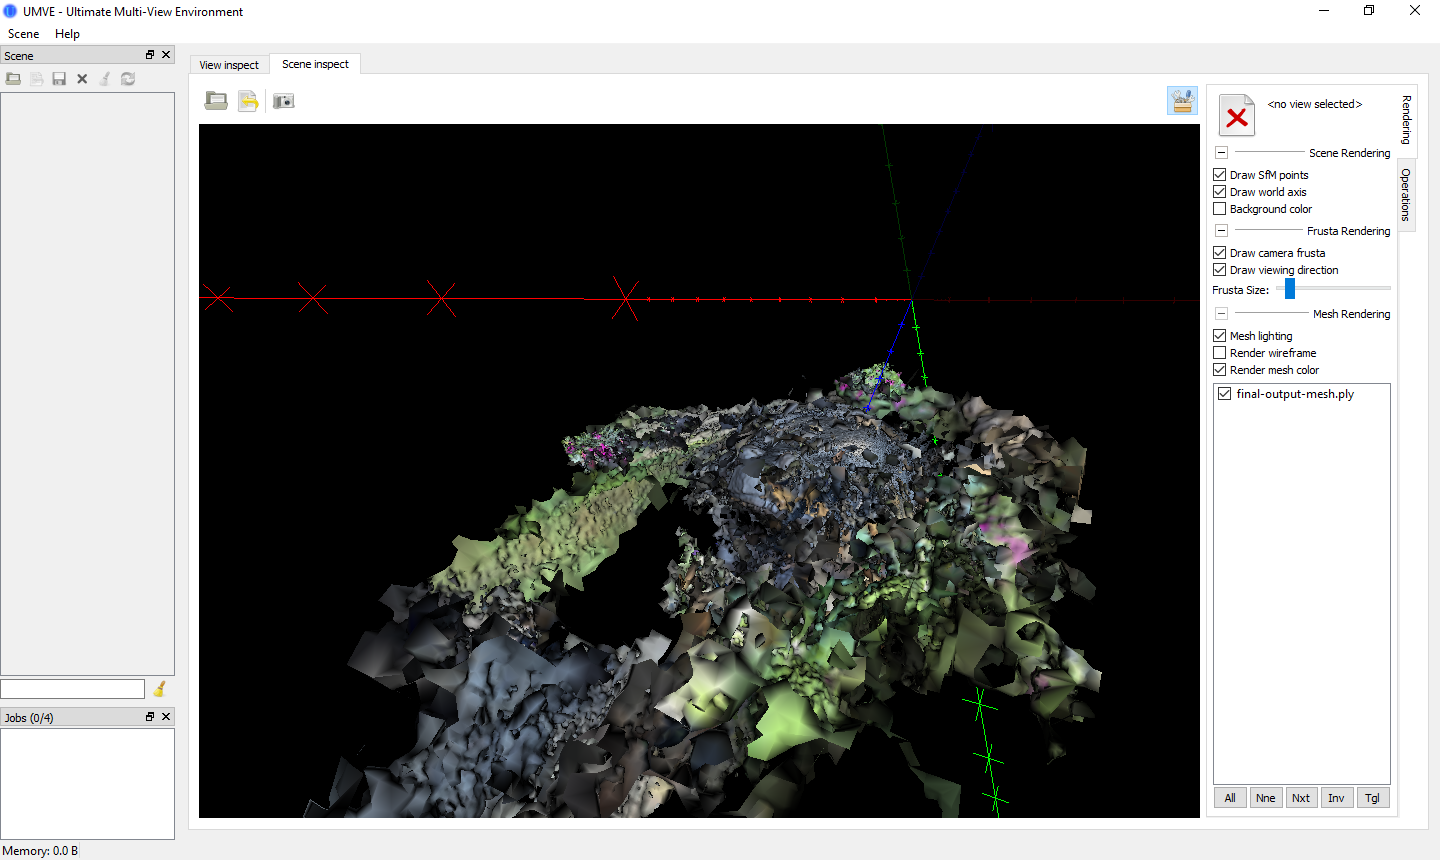
\includegraphics[width=1\linewidth]{figs/mvemeshout.png}
% 	\caption{%
% 	Malha com ruídos proveniente do comando \emph{fssrecon}.
% 	%\cite{Cui:Theobalt:etal:PAMI2013,Pajdla:etal:ICCV2011}.
% 	}\label{fig:MVEFSSRMesh}
% \end{figure} 

% Finalmente, basta limpar a malha atual com o comando \emph{meshclean}, onde foi obtido o resultado \ref{MVEMeshClean}.

% \begin{figure}[!h]
% 	\centering
% 	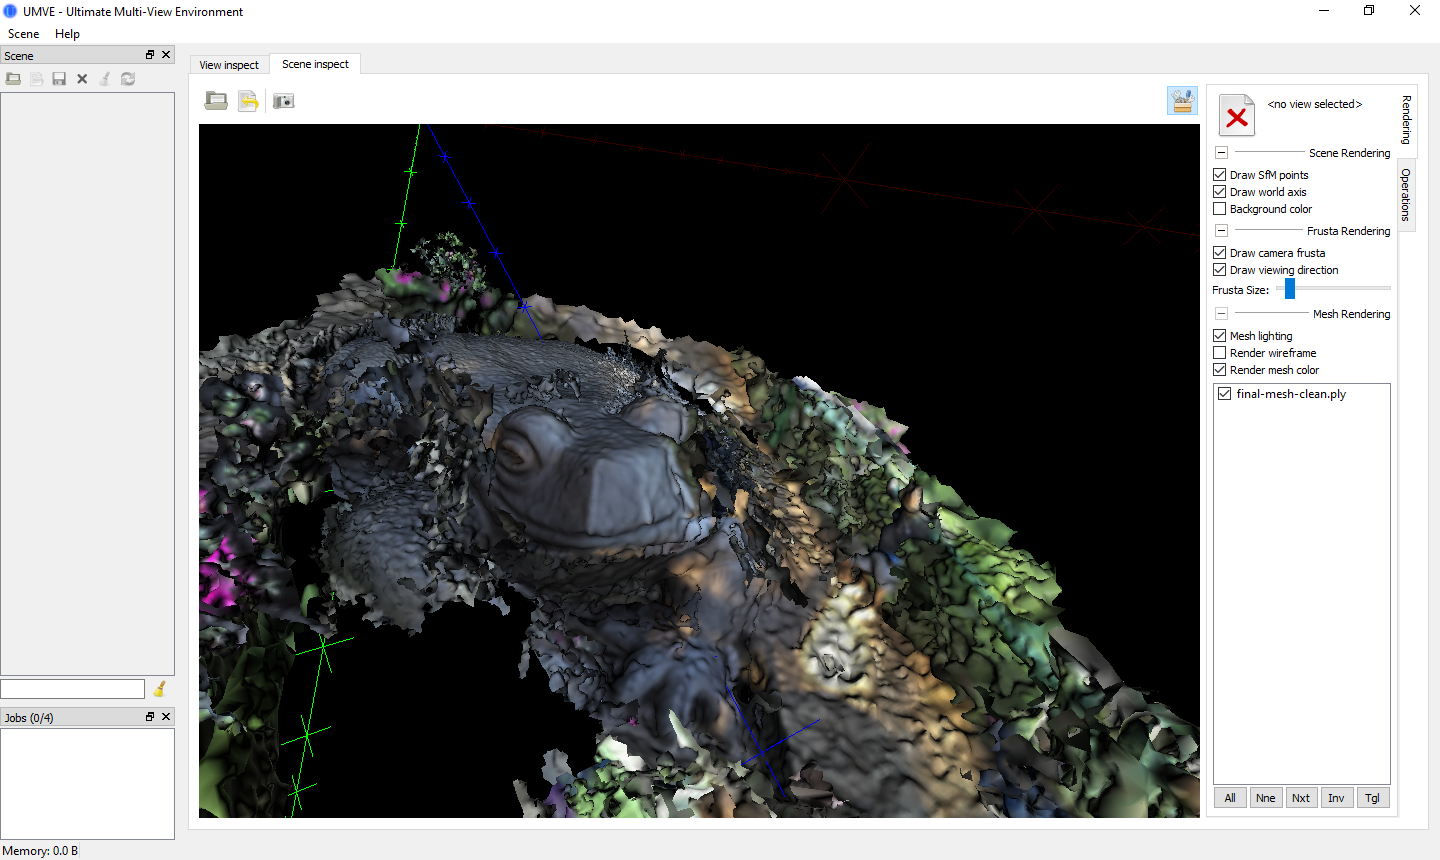
\includegraphics[width=1\linewidth]{figs/mvemeshclean.png}
% 	\caption{%
% 	Resultado final, após a remoção dos ruídos da malha.
% 	%\cite{Cui:Theobalt:etal:PAMI2013,Pajdla:etal:ICCV2011}.
% 	}\label{fig:MVEMeshClean}
% \end{figure} 